% Options for packages loaded elsewhere
\PassOptionsToPackage{unicode}{hyperref}
\PassOptionsToPackage{hyphens}{url}
%
\documentclass[
]{article}
\usepackage{amsmath,amssymb}
\usepackage{iftex}
\ifPDFTeX
  \usepackage[T1]{fontenc}
  \usepackage[utf8]{inputenc}
  \usepackage{textcomp} % provide euro and other symbols
\else % if luatex or xetex
  \usepackage{unicode-math} % this also loads fontspec
  \defaultfontfeatures{Scale=MatchLowercase}
  \defaultfontfeatures[\rmfamily]{Ligatures=TeX,Scale=1}
\fi
\usepackage{lmodern}
\ifPDFTeX\else
  % xetex/luatex font selection
\fi
% Use upquote if available, for straight quotes in verbatim environments
\IfFileExists{upquote.sty}{\usepackage{upquote}}{}
\IfFileExists{microtype.sty}{% use microtype if available
  \usepackage[]{microtype}
  \UseMicrotypeSet[protrusion]{basicmath} % disable protrusion for tt fonts
}{}
\makeatletter
\@ifundefined{KOMAClassName}{% if non-KOMA class
  \IfFileExists{parskip.sty}{%
    \usepackage{parskip}
  }{% else
    \setlength{\parindent}{0pt}
    \setlength{\parskip}{6pt plus 2pt minus 1pt}}
}{% if KOMA class
  \KOMAoptions{parskip=half}}
\makeatother
\usepackage{xcolor}
\usepackage[margin=1in]{geometry}
\usepackage{color}
\usepackage{fancyvrb}
\newcommand{\VerbBar}{|}
\newcommand{\VERB}{\Verb[commandchars=\\\{\}]}
\DefineVerbatimEnvironment{Highlighting}{Verbatim}{commandchars=\\\{\}}
% Add ',fontsize=\small' for more characters per line
\usepackage{framed}
\definecolor{shadecolor}{RGB}{248,248,248}
\newenvironment{Shaded}{\begin{snugshade}}{\end{snugshade}}
\newcommand{\AlertTok}[1]{\textcolor[rgb]{0.94,0.16,0.16}{#1}}
\newcommand{\AnnotationTok}[1]{\textcolor[rgb]{0.56,0.35,0.01}{\textbf{\textit{#1}}}}
\newcommand{\AttributeTok}[1]{\textcolor[rgb]{0.13,0.29,0.53}{#1}}
\newcommand{\BaseNTok}[1]{\textcolor[rgb]{0.00,0.00,0.81}{#1}}
\newcommand{\BuiltInTok}[1]{#1}
\newcommand{\CharTok}[1]{\textcolor[rgb]{0.31,0.60,0.02}{#1}}
\newcommand{\CommentTok}[1]{\textcolor[rgb]{0.56,0.35,0.01}{\textit{#1}}}
\newcommand{\CommentVarTok}[1]{\textcolor[rgb]{0.56,0.35,0.01}{\textbf{\textit{#1}}}}
\newcommand{\ConstantTok}[1]{\textcolor[rgb]{0.56,0.35,0.01}{#1}}
\newcommand{\ControlFlowTok}[1]{\textcolor[rgb]{0.13,0.29,0.53}{\textbf{#1}}}
\newcommand{\DataTypeTok}[1]{\textcolor[rgb]{0.13,0.29,0.53}{#1}}
\newcommand{\DecValTok}[1]{\textcolor[rgb]{0.00,0.00,0.81}{#1}}
\newcommand{\DocumentationTok}[1]{\textcolor[rgb]{0.56,0.35,0.01}{\textbf{\textit{#1}}}}
\newcommand{\ErrorTok}[1]{\textcolor[rgb]{0.64,0.00,0.00}{\textbf{#1}}}
\newcommand{\ExtensionTok}[1]{#1}
\newcommand{\FloatTok}[1]{\textcolor[rgb]{0.00,0.00,0.81}{#1}}
\newcommand{\FunctionTok}[1]{\textcolor[rgb]{0.13,0.29,0.53}{\textbf{#1}}}
\newcommand{\ImportTok}[1]{#1}
\newcommand{\InformationTok}[1]{\textcolor[rgb]{0.56,0.35,0.01}{\textbf{\textit{#1}}}}
\newcommand{\KeywordTok}[1]{\textcolor[rgb]{0.13,0.29,0.53}{\textbf{#1}}}
\newcommand{\NormalTok}[1]{#1}
\newcommand{\OperatorTok}[1]{\textcolor[rgb]{0.81,0.36,0.00}{\textbf{#1}}}
\newcommand{\OtherTok}[1]{\textcolor[rgb]{0.56,0.35,0.01}{#1}}
\newcommand{\PreprocessorTok}[1]{\textcolor[rgb]{0.56,0.35,0.01}{\textit{#1}}}
\newcommand{\RegionMarkerTok}[1]{#1}
\newcommand{\SpecialCharTok}[1]{\textcolor[rgb]{0.81,0.36,0.00}{\textbf{#1}}}
\newcommand{\SpecialStringTok}[1]{\textcolor[rgb]{0.31,0.60,0.02}{#1}}
\newcommand{\StringTok}[1]{\textcolor[rgb]{0.31,0.60,0.02}{#1}}
\newcommand{\VariableTok}[1]{\textcolor[rgb]{0.00,0.00,0.00}{#1}}
\newcommand{\VerbatimStringTok}[1]{\textcolor[rgb]{0.31,0.60,0.02}{#1}}
\newcommand{\WarningTok}[1]{\textcolor[rgb]{0.56,0.35,0.01}{\textbf{\textit{#1}}}}
\usepackage{graphicx}
\makeatletter
\def\maxwidth{\ifdim\Gin@nat@width>\linewidth\linewidth\else\Gin@nat@width\fi}
\def\maxheight{\ifdim\Gin@nat@height>\textheight\textheight\else\Gin@nat@height\fi}
\makeatother
% Scale images if necessary, so that they will not overflow the page
% margins by default, and it is still possible to overwrite the defaults
% using explicit options in \includegraphics[width, height, ...]{}
\setkeys{Gin}{width=\maxwidth,height=\maxheight,keepaspectratio}
% Set default figure placement to htbp
\makeatletter
\def\fps@figure{htbp}
\makeatother
\setlength{\emergencystretch}{3em} % prevent overfull lines
\providecommand{\tightlist}{%
  \setlength{\itemsep}{0pt}\setlength{\parskip}{0pt}}
\setcounter{secnumdepth}{5}
\usepackage[spanish]{babel}
\usepackage{fontspec}
\ifLuaTeX
  \usepackage{selnolig}  % disable illegal ligatures
\fi
\IfFileExists{bookmark.sty}{\usepackage{bookmark}}{\usepackage{hyperref}}
\IfFileExists{xurl.sty}{\usepackage{xurl}}{} % add URL line breaks if available
\urlstyle{same}
\hypersetup{
  pdftitle={Tarea 2},
  pdfauthor={José Ignacio Rojas Zárate, C16911; Montserrat Beirute Abarca, C10997; Valeria Vásquez Venegas, C18373},
  hidelinks,
  pdfcreator={LaTeX via pandoc}}

\title{Tarea 2}
\usepackage{etoolbox}
\makeatletter
\providecommand{\subtitle}[1]{% add subtitle to \maketitle
  \apptocmd{\@title}{\par {\large #1 \par}}{}{}
}
\makeatother
\subtitle{Estadística Actuarial II}
\author{José Ignacio Rojas Zárate, C16911 \and Montserrat Beirute
Abarca, C10997 \and Valeria Vásquez Venegas, C18373}
\date{07 de febrero de 2024}

\begin{document}
\maketitle

{
\setcounter{tocdepth}{2}
\tableofcontents
}
\newpage

\hypertarget{ejercicio-1}{%
\section{Ejercicio 1}\label{ejercicio-1}}

\textbf{Usando un algoritmo de integración por Montecarlo estime ln(2)
con un error absoluto de 10−3}

Considere la siguiente integral:
\[ \int_{0}^{1} \frac{\ln(x + 1)}{2} + \frac{1}{2} \, dx \].

\emph{Solución:}

Empezamos separando la integral en dos partes. Para
\(\int \frac{\ln(x + 1)}{2} \, dx\): Realizamos la sustitución
\(u = x + 1\) y \(du = dx\). Note que si
\(x \rightarrow 0 \Rightarrow u \rightarrow 1\) y si
\(x \rightarrow 1 \Rightarrow u \rightarrow 2\). Esta primera integral
se convierte en: \(\frac{1}{2} \int_{1}^{2} \ln(u) \, du\)

Ahora, se aplica la regla de integración por partes, donde
\(m = \ln(u) \Rightarrow dm = \frac{1}{u} du\) y
\(dv = 1 \Rightarrow v = u\):

\[ \frac{1}{2} \left( u \ln(u) \Big|_{1}^2 - \int_{1}^{2} u \, \frac{1}{u} du\right) \]

Esto se simplifica a:
\(\frac{1}{2} \left(\ln(2) - 1 \right) = \frac{\ln(2)}{2} - \frac{1}{2}\).

La otra parte de la integral original,
\(\int_{0}^{1} \frac{1}{2} \, dx = \frac{1}{2}\):

Por lo tanto, la solución a la integral es
\(\frac{\ln(2)}{2} - \frac{1}{2} + \frac{1}{2} = \ln(2)\).

Ahora, procedemos a aplicar el algoritmo de Montecarlo:

\begin{Shaded}
\begin{Highlighting}[]
\FunctionTok{set.seed}\NormalTok{(}\DecValTok{147}\NormalTok{) }\CommentTok{\# definimos una semilla}
\NormalTok{n }\OtherTok{\textless{}{-}}\DecValTok{10}\SpecialCharTok{\^{}}\DecValTok{4} \CommentTok{\# tamaño de la muestra}
\NormalTok{U }\OtherTok{\textless{}{-}}\FunctionTok{runif}\NormalTok{(n) }\CommentTok{\# genera un vector con distribución uniforme}

\NormalTok{g }\OtherTok{\textless{}{-}}\FunctionTok{Vectorize}\NormalTok{(}\ControlFlowTok{function}\NormalTok{(x) (}\FunctionTok{log}\NormalTok{(x }\SpecialCharTok{+} \DecValTok{1}\NormalTok{)}\SpecialCharTok{/}\DecValTok{2}\NormalTok{) }\SpecialCharTok{+}\NormalTok{ (}\DecValTok{1}\SpecialCharTok{/}\DecValTok{2}\NormalTok{) ) }\CommentTok{\# construimos la función g }

\FunctionTok{curve}\NormalTok{(g,}\DecValTok{0}\NormalTok{,}\DecValTok{1}\NormalTok{,}\AttributeTok{col=}\StringTok{"lightblue4"}\NormalTok{,}\AttributeTok{lwd=}\DecValTok{1}\NormalTok{,}\AttributeTok{main=}\StringTok{"Gráfico de g(X)"}\NormalTok{)}
\FunctionTok{grid}\NormalTok{()  }
\end{Highlighting}
\end{Shaded}

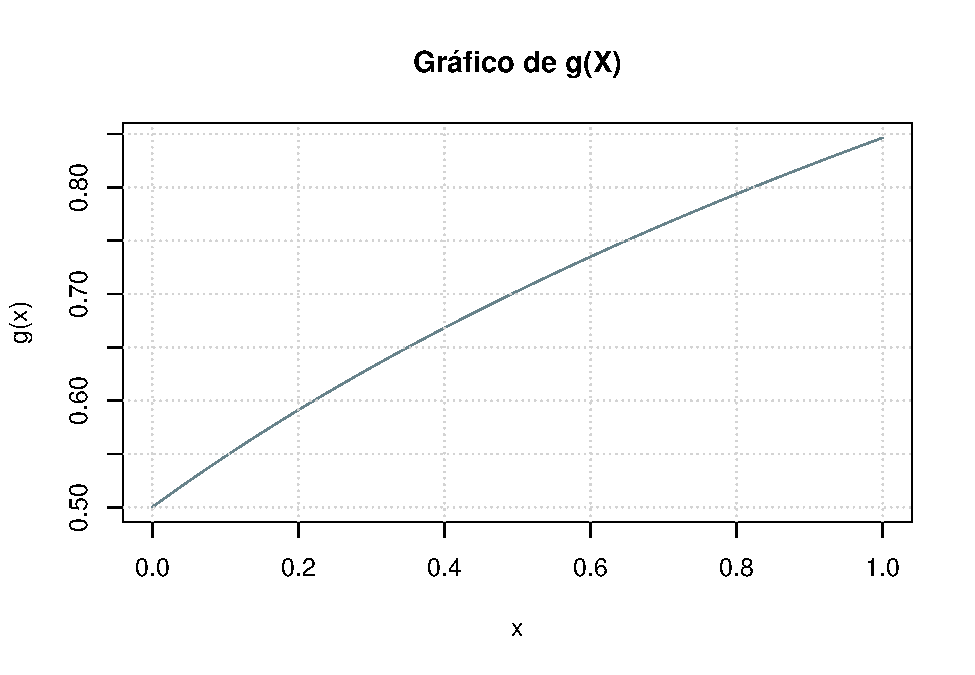
\includegraphics{tarea2_files/figure-latex/unnamed-chunk-2-1.pdf}

\begin{Shaded}
\begin{Highlighting}[]
\NormalTok{Y }\OtherTok{\textless{}{-}} \FunctionTok{g}\NormalTok{(U) }\CommentTok{\#genera el vector para cada observación}
\NormalTok{acumulado}\OtherTok{\textless{}{-}}\FunctionTok{cumsum}\NormalTok{(Y)}\SpecialCharTok{/}\NormalTok{(}\DecValTok{1}\SpecialCharTok{:}\NormalTok{n)}
\FunctionTok{plot}\NormalTok{(}\DecValTok{1}\SpecialCharTok{:}\NormalTok{n,acumulado,}\AttributeTok{col=}\StringTok{"lightblue4"}\NormalTok{,}\AttributeTok{type=}\StringTok{"l"}\NormalTok{,}\AttributeTok{ylab=}\StringTok{"Aproximación"}\NormalTok{,}\AttributeTok{xlab=}\StringTok{"Iteraciones"}\NormalTok{)}
\FunctionTok{abline}\NormalTok{(}\AttributeTok{h=}\FunctionTok{integrate}\NormalTok{(g,}\DecValTok{0}\NormalTok{,}\DecValTok{1}\NormalTok{)}\SpecialCharTok{$}\NormalTok{value,}\AttributeTok{col=}\StringTok{"coral2"}\NormalTok{,}\AttributeTok{lwd=}\DecValTok{1}\NormalTok{)}
\end{Highlighting}
\end{Shaded}

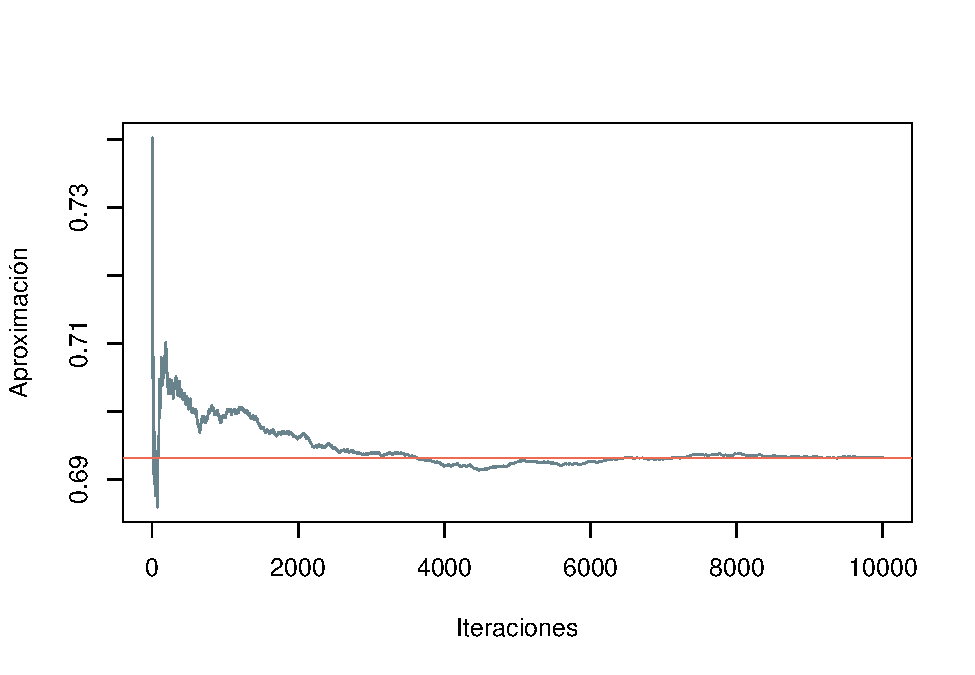
\includegraphics{tarea2_files/figure-latex/unnamed-chunk-2-2.pdf}

\begin{Shaded}
\begin{Highlighting}[]
\NormalTok{P\_est1}\OtherTok{=}\FunctionTok{mean}\NormalTok{(Y)}

\NormalTok{e1 }\OtherTok{\textless{}{-}}\NormalTok{(}\FunctionTok{abs}\NormalTok{(P\_est1}\SpecialCharTok{{-}}\FunctionTok{log}\NormalTok{(}\DecValTok{2}\NormalTok{)))}
\end{Highlighting}
\end{Shaded}

\begin{Shaded}
\begin{Highlighting}[]
\NormalTok{e1}
\end{Highlighting}
\end{Shaded}

\begin{verbatim}
## [1] 4.587881e-05
\end{verbatim}

Concluya que con la función considerada, el algrotimo de integración por
Montecarlo arroja un error absoluto de 4.587881e-05 al estimar ln(2).

\newpage

\hypertarget{ejercicio-2}{%
\section{Ejercicio 2}\label{ejercicio-2}}

\textbf{Usando la metodología de Muestreo por Importancia, si }
\(X \sim N(0.5,0.5)\) \textbf{estime:}

\begin{enumerate}
\def\labelenumi{\alph{enumi}.}
\tightlist
\item
  \(P(X \leq -5)\)
\end{enumerate}

\begin{Shaded}
\begin{Highlighting}[]
\FunctionTok{pnorm}\NormalTok{(}\DecValTok{6}\NormalTok{,}\AttributeTok{mean =} \FloatTok{0.5}\NormalTok{,}\AttributeTok{sd =}\NormalTok{ (}\FloatTok{0.5}\SpecialCharTok{\^{}}\NormalTok{(}\DecValTok{1}\SpecialCharTok{/}\DecValTok{2}\NormalTok{)),}\AttributeTok{lower.tail =}\NormalTok{ F)}
\end{Highlighting}
\end{Shaded}

\begin{verbatim}
## [1] 3.678924e-15
\end{verbatim}

Concluya que la \(P(X \leq -5) = 3.678924e-15\).

\begin{enumerate}
\def\labelenumi{\alph{enumi}.}
\setcounter{enumi}{1}
\tightlist
\item
  Estime el error absoluto de la estimación del punto a:
\end{enumerate}

\begin{Shaded}
\begin{Highlighting}[]
\NormalTok{n }\OtherTok{\textless{}{-}}\DecValTok{10}\SpecialCharTok{\^{}}\DecValTok{4} \CommentTok{\# Tamaño de la muestra}
\NormalTok{A }\OtherTok{\textless{}{-}}\FunctionTok{rexp}\NormalTok{(n) }\SpecialCharTok{+} \DecValTok{6}

\NormalTok{g }\OtherTok{\textless{}{-}}\FunctionTok{Vectorize}\NormalTok{(}\ControlFlowTok{function}\NormalTok{(x) ((}\DecValTok{1}\SpecialCharTok{/}\NormalTok{pi) }\SpecialCharTok{*} \FunctionTok{exp}\NormalTok{(}\SpecialCharTok{{-}}\NormalTok{(x}\FloatTok{{-}0.5}\NormalTok{)}\SpecialCharTok{\^{}}\DecValTok{2}\NormalTok{)}\SpecialCharTok{/}\NormalTok{(}\FunctionTok{exp}\NormalTok{(}\SpecialCharTok{{-}}\NormalTok{x}\SpecialCharTok{+}\DecValTok{6}\NormalTok{))))}

\NormalTok{Y2}\OtherTok{\textless{}{-}}\FunctionTok{g}\NormalTok{(A)}

\NormalTok{M}\OtherTok{\textless{}{-}}\FunctionTok{matrix}\NormalTok{(}\FunctionTok{c}\NormalTok{(}\FunctionTok{mean}\NormalTok{(Y2),}\FunctionTok{pnorm}\NormalTok{(}\DecValTok{6}\NormalTok{,}\AttributeTok{mean =} \FloatTok{0.5}\NormalTok{,}\AttributeTok{sd =}\NormalTok{ (}\FloatTok{0.5}\SpecialCharTok{\^{}}\NormalTok{(}\DecValTok{1}\SpecialCharTok{/}\DecValTok{2}\NormalTok{)), }\AttributeTok{lower.tail =}\NormalTok{ F),}
            \FunctionTok{abs}\NormalTok{(}\FunctionTok{mean}\NormalTok{(Y2)}\SpecialCharTok{{-}}\FunctionTok{pnorm}\NormalTok{(}\DecValTok{6}\NormalTok{,}\AttributeTok{mean =} \FloatTok{0.5}\NormalTok{,}\AttributeTok{sd =}\NormalTok{ (}\FloatTok{0.5}\SpecialCharTok{\^{}}\NormalTok{(}\DecValTok{1}\SpecialCharTok{/}\DecValTok{2}\NormalTok{)), }\AttributeTok{lower.tail =}\NormalTok{ F)),}
            \FunctionTok{sqrt}\NormalTok{(}\FunctionTok{var}\NormalTok{(Y2)}\SpecialCharTok{/}\FunctionTok{sqrt}\NormalTok{(}\DecValTok{10}\SpecialCharTok{\^{}}\DecValTok{4}\NormalTok{))),}\AttributeTok{ncol=}\DecValTok{4}\NormalTok{, }\AttributeTok{byrow=}\ConstantTok{TRUE}\NormalTok{)}

\FunctionTok{colnames}\NormalTok{(M) }\OtherTok{\textless{}{-}} \FunctionTok{c}\NormalTok{(}\StringTok{"Estimacion"}\NormalTok{, }\StringTok{"Valor Real"}\NormalTok{,}\StringTok{"Error Absoluto"}\NormalTok{,}\StringTok{"Error Estandar"}\NormalTok{)}

\NormalTok{M}
\end{Highlighting}
\end{Shaded}

\begin{verbatim}
##        Estimacion   Valor Real Error Absoluto Error Estandar
## [1,] 2.056013e-15 3.678924e-15   1.622911e-15   4.619617e-16
\end{verbatim}

Conculuya que el error absoluto es de 1.622911e-15 al utilizar la
metodología de Muestreo por Importancia.

\newpage

\hypertarget{ejercicio-5}{%
\section{Ejercicio 5}\label{ejercicio-5}}

\textbf{Una aseguradora tiene un producto llamado Doble Seguro de Vida
(DSV) el cual paga 2 veces la suma asegurada si la persona fallece antes
de los 60 años, paga 1 suma asegurada cuando la persona cumple los 60
años (si no ha fallecido) y paga 1 suma asegurada si fallece después de
los 60 años.}\\
\textbf{Construya con la ayuda de un MCMC la distribución de los pagos
por año de que se espera de este seguro. Use al menos 10 000
iteraciones. Y muestre Histograma.}

Primero abrimos la base de datos de mortalidad, luego filtramos para
obtener los datos de un hombre nacido en 1994.

\begin{Shaded}
\begin{Highlighting}[]
\NormalTok{tabla\_vida\_original }\OtherTok{\textless{}{-}} \FunctionTok{read\_excel}\NormalTok{(}\StringTok{"tabla.xls"}\NormalTok{)}

\CommentTok{\#filtrando por año de nacimiento y edad}
\NormalTok{tabla\_vida }\OtherTok{\textless{}{-}}\NormalTok{ tabla\_vida\_original[(tabla\_vida\_original}\SpecialCharTok{$}\NormalTok{ynac }\SpecialCharTok{==} \DecValTok{1994}\NormalTok{) }\SpecialCharTok{\&} 
\NormalTok{                                    (tabla\_vida\_original}\SpecialCharTok{$}\NormalTok{sex }\SpecialCharTok{==} \DecValTok{1}\NormalTok{),] }
\end{Highlighting}
\end{Shaded}

Para realizar la simulación primero definimos algunos aspectos como
semilla, numero de iteraciones, vector de mortalidad (filtrado para
mortalidades de 30 años en adelante), longitud del vector y un vector
vacio donde almacenar los resultados.

\begin{Shaded}
\begin{Highlighting}[]
\FunctionTok{set.seed}\NormalTok{(}\DecValTok{2024}\NormalTok{)}
\NormalTok{iteraciones }\OtherTok{\textless{}{-}} \DecValTok{10}\SpecialCharTok{\^{}}\DecValTok{4}
\NormalTok{vec\_qx }\OtherTok{\textless{}{-}}\NormalTok{ tabla\_vida}\SpecialCharTok{$}\NormalTok{qx[}\DecValTok{25}\SpecialCharTok{:}\FunctionTok{length}\NormalTok{(tabla\_vida}\SpecialCharTok{$}\NormalTok{qx)]}
\NormalTok{n }\OtherTok{\textless{}{-}} \FunctionTok{length}\NormalTok{(vec\_qx)}
\NormalTok{vec\_resultados}\OtherTok{\textless{}{-}}\FunctionTok{rep}\NormalTok{(}\DecValTok{0}\NormalTok{,iteraciones)}

\ControlFlowTok{for}\NormalTok{(i }\ControlFlowTok{in} \FunctionTok{c}\NormalTok{(}\DecValTok{1}\SpecialCharTok{:}\NormalTok{iteraciones))\{}
\NormalTok{  U}\OtherTok{\textless{}{-}}\FunctionTok{runif}\NormalTok{(n)}
\NormalTok{  t }\OtherTok{\textless{}{-}} \DecValTok{1}
\NormalTok{  cont }\OtherTok{\textless{}{-}} \DecValTok{1}
  \ControlFlowTok{while}\NormalTok{(t }\SpecialCharTok{==} \DecValTok{1}\NormalTok{)\{}
    \ControlFlowTok{if}\NormalTok{(U[cont]}\SpecialCharTok{\textgreater{}}\NormalTok{vec\_qx[cont]) }\CommentTok{\#Aqui se decide si la persona sobrevive o muere}
\NormalTok{      \{cont}\OtherTok{\textless{}{-}}\NormalTok{cont}\SpecialCharTok{+}\DecValTok{1}
\NormalTok{    \}}\ControlFlowTok{else}\NormalTok{\{}
\NormalTok{      t}\OtherTok{\textless{}{-}}\DecValTok{0}
\NormalTok{      \}}
\NormalTok{  \}}
\NormalTok{  vec\_resultados[i]}\OtherTok{\textless{}{-}}\NormalTok{cont}\DecValTok{{-}1}
\NormalTok{\}}
\end{Highlighting}
\end{Shaded}

Ahora podemos observar la distribución de muertes:

\begin{Shaded}
\begin{Highlighting}[]
\FunctionTok{plot}\NormalTok{(}\FunctionTok{density}\NormalTok{(vec\_resultados))}
\end{Highlighting}
\end{Shaded}

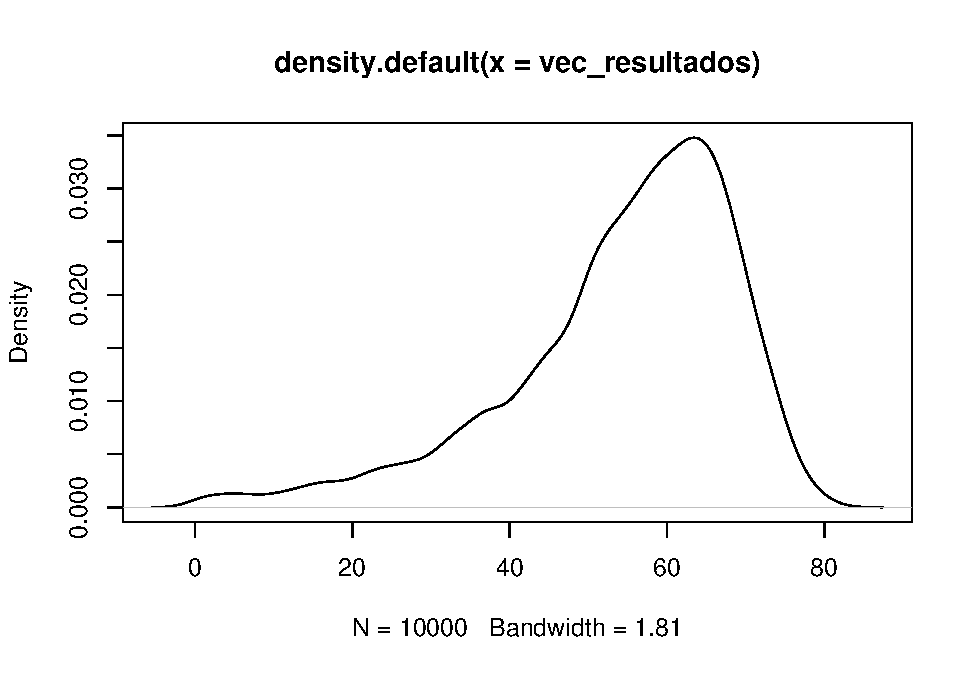
\includegraphics{tarea2_files/figure-latex/unnamed-chunk-8-1.pdf}

Para poder obtener la distribución de pagos por año, lo que hacemos es
considerar que cada muerte después de 30 años (60 años del individuo)
representa un pago, pero si la persona muere antes de los próximos 30
años se consideran 2 pagos, por lo que añadimos una observación extra en
ese caso.

\begin{Shaded}
\begin{Highlighting}[]
\ControlFlowTok{for}\NormalTok{ (i }\ControlFlowTok{in} \DecValTok{1}\SpecialCharTok{:}\FunctionTok{length}\NormalTok{(vec\_resultados))\{}
  \ControlFlowTok{if}\NormalTok{(vec\_resultados[i] }\SpecialCharTok{\textless{}}\NormalTok{ (}\DecValTok{60{-}30}\NormalTok{))\{}
\NormalTok{    vec\_resultados }\OtherTok{\textless{}{-}} \FunctionTok{c}\NormalTok{(vec\_resultados, vec\_resultados[i])}
\NormalTok{  \}}
\NormalTok{\}}
\end{Highlighting}
\end{Shaded}

Graficando el resultado:

\begin{Shaded}
\begin{Highlighting}[]
\FunctionTok{plot}\NormalTok{(}\FunctionTok{density}\NormalTok{(vec\_resultados))}
\end{Highlighting}
\end{Shaded}

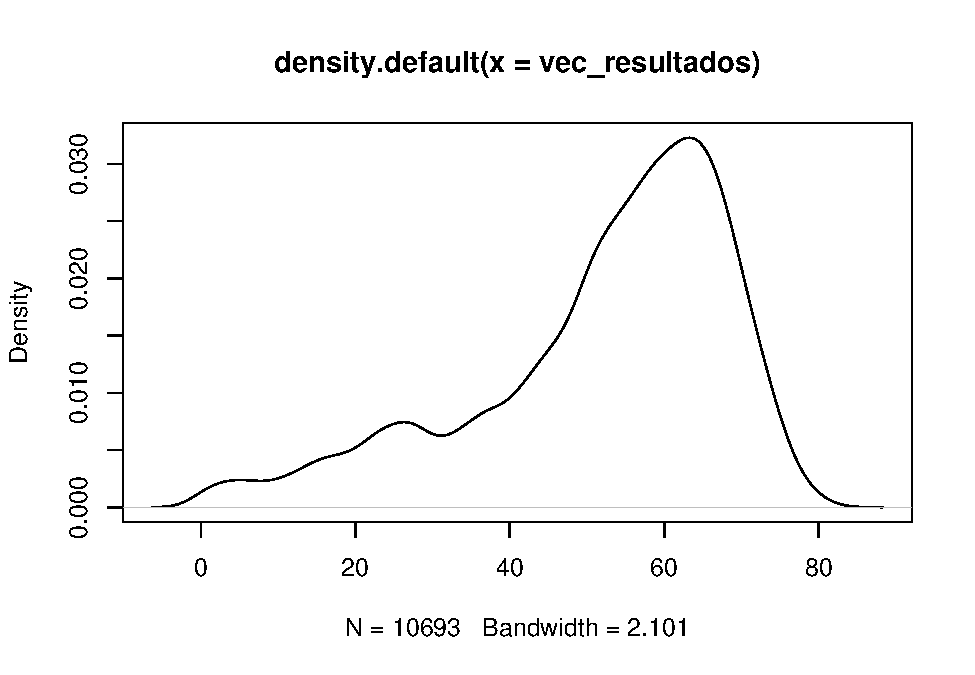
\includegraphics{tarea2_files/figure-latex/unnamed-chunk-10-1.pdf}

\newpage

\hypertarget{ejercicio-6}{%
\section{Ejercicio 6}\label{ejercicio-6}}

\textbf{Usando el Algoritmo de Metropolis-Hastings construya una muestra
de} \(Z=X_1−X_2\) \textbf{donde }\(𝑋_1\sim𝑁(𝜇,𝜎^2)\) \textbf{y}
\(𝑋_2\sim𝑁(𝜇/2,𝜎^2/4)\)\textbf{, considere para este ejercicio}
\(𝜇=𝜎=4\).

\begin{enumerate}
\def\labelenumi{\alph{enumi}.}
\tightlist
\item
  Gráfique la distribución de \(𝑍\) junto con las medias de
  \(𝑋_1\),\(𝑋_2\).
\end{enumerate}

Primero definiremos los parámetros \(𝜇=𝜎=4\), además, como
\(Z=X_1−X_2\), entonces \(Z\) sigue una distribución
\(Z\sim𝑁(𝜇-𝜇/2,𝜎^2+𝜎^2/4)\). Luego definimos la funcion fPI.

\begin{Shaded}
\begin{Highlighting}[]
\NormalTok{mu }\OtherTok{\textless{}{-}} \DecValTok{4}
\NormalTok{sigma }\OtherTok{\textless{}{-}} \DecValTok{4}

\NormalTok{mu\_z }\OtherTok{\textless{}{-}} \DecValTok{4}\SpecialCharTok{{-}}\NormalTok{(}\DecValTok{4}\SpecialCharTok{/}\DecValTok{2}\NormalTok{)}
\NormalTok{sigma\_z }\OtherTok{\textless{}{-}} \DecValTok{4}\SpecialCharTok{+}\NormalTok{(}\DecValTok{4}\SpecialCharTok{/}\DecValTok{4}\NormalTok{) }\CommentTok{\#En realidad es sigma\^{}2}

\NormalTok{fPI }\OtherTok{=} \ControlFlowTok{function}\NormalTok{(x)}
\NormalTok{\{}
\NormalTok{  fx }\OtherTok{=} \FunctionTok{exp}\NormalTok{( }\SpecialCharTok{{-}}\NormalTok{((x }\SpecialCharTok{{-}}\NormalTok{ mu\_z)}\SpecialCharTok{\^{}}\DecValTok{2}\SpecialCharTok{/}\NormalTok{(}\DecValTok{2}\SpecialCharTok{*}\NormalTok{(sigma\_z))))}\SpecialCharTok{/}\NormalTok{(}\FunctionTok{sqrt}\NormalTok{(}\DecValTok{2}\SpecialCharTok{*}\NormalTok{pi}\SpecialCharTok{*}\NormalTok{sigma\_z))}
  \FunctionTok{return}\NormalTok{(fx)}
\NormalTok{\}}
\end{Highlighting}
\end{Shaded}

Ahora podemos mostrar la distribución de \(Z\):

\begin{Shaded}
\begin{Highlighting}[]
\FunctionTok{curve}\NormalTok{(}\FunctionTok{fPI}\NormalTok{(x), }\AttributeTok{from=}\SpecialCharTok{{-}}\DecValTok{5}\NormalTok{,}\AttributeTok{to=}\DecValTok{9}\NormalTok{, }\AttributeTok{main=}\StringTok{"Distribucion de Z"}\NormalTok{,}\AttributeTok{xlab=}\StringTok{"x"}\NormalTok{,}\AttributeTok{ylab=}\StringTok{"f(x)"}\NormalTok{)}
\FunctionTok{abline}\NormalTok{(}\AttributeTok{v =} \DecValTok{4}\NormalTok{, }\AttributeTok{lty =} \DecValTok{3}\NormalTok{) }\CommentTok{\#Media de x1}
\FunctionTok{abline}\NormalTok{(}\AttributeTok{v =} \DecValTok{2}\NormalTok{, }\AttributeTok{lty =} \DecValTok{3}\NormalTok{) }\CommentTok{\#Media de x2}
\end{Highlighting}
\end{Shaded}

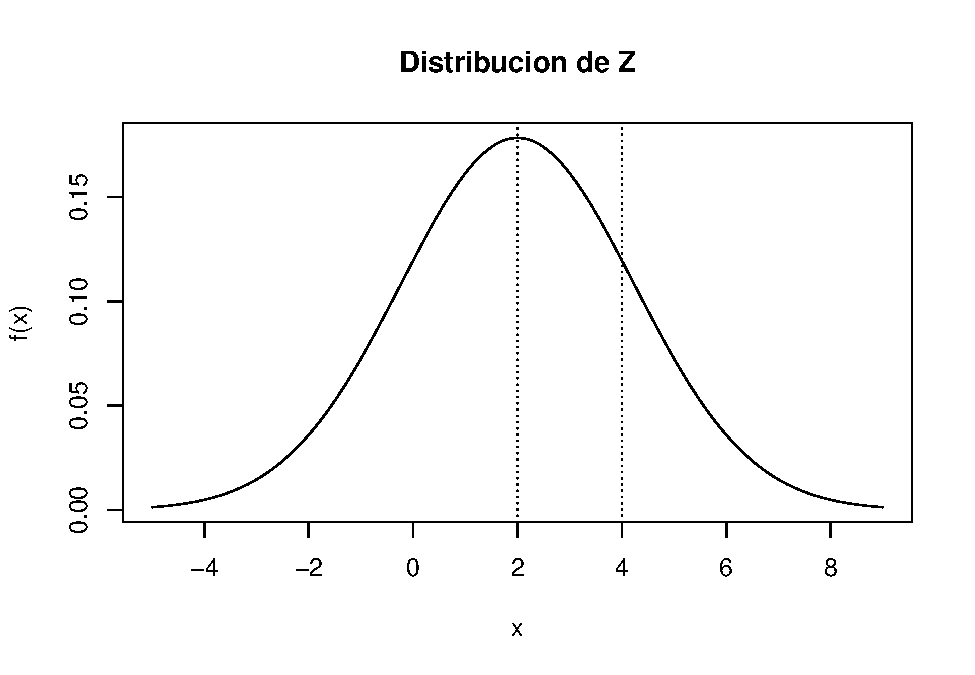
\includegraphics{tarea2_files/figure-latex/unnamed-chunk-12-1.pdf}

\begin{enumerate}
\def\labelenumi{\alph{enumi}.}
\setcounter{enumi}{1}
\tightlist
\item
  Gráfique la distribución (histograma) de la muestra MCMC del algoritmo
  junto con las medias de \(𝑋_1\),\(𝑋_2\).
\end{enumerate}

Primero definimos la funcion fpK y luego aplicamos el algoritmo

\begin{Shaded}
\begin{Highlighting}[]
\CommentTok{\#Usaremos dist cauchy para el proceso de markov}
\NormalTok{fpK }\OtherTok{=} \ControlFlowTok{function}\NormalTok{(x,y)\{}
\NormalTok{  pK }\OtherTok{=} \FunctionTok{dcauchy}\NormalTok{(y,}\AttributeTok{location =}\NormalTok{ x) }\CommentTok{\#x es el centro del pico de la distribución.}
  \FunctionTok{return}\NormalTok{(pK)}
\NormalTok{\}}

\CommentTok{\#Aplicando el algoritmo}
\NormalTok{N }\OtherTok{=} \DecValTok{10}\SpecialCharTok{\^{}}\DecValTok{5} \CommentTok{\# Número de Iteraciones}
\NormalTok{L }\OtherTok{=} \DecValTok{1000} \CommentTok{\# periodo quemado (burn in)}

\NormalTok{MCMC }\OtherTok{=} \FunctionTok{matrix}\NormalTok{(}\AttributeTok{data =} \DecValTok{0}\NormalTok{, }\AttributeTok{nrow =}\NormalTok{ N, }\AttributeTok{ncol =} \DecValTok{12}\NormalTok{)}
\FunctionTok{colnames}\NormalTok{(MCMC) }\OtherTok{=}
  \FunctionTok{c}\NormalTok{(}\StringTok{"x"}\NormalTok{,}\StringTok{"y"}\NormalTok{,}\StringTok{"PIx"}\NormalTok{,}\StringTok{"PIy"}\NormalTok{,}\StringTok{"Kxy"}\NormalTok{,}\StringTok{"Kyx"}\NormalTok{,}\StringTok{"Rxy"}\NormalTok{,}\StringTok{"Ryx"}\NormalTok{,}\StringTok{"Mxy"}\NormalTok{,}\StringTok{"Myx"}\NormalTok{,}\StringTok{"Fxy"}\NormalTok{,}\StringTok{"Salto"}\NormalTok{)}
\CommentTok{\# 1. Inicial con un valor arbitrario de x del dominio de distribución}
\NormalTok{x }\OtherTok{=} \FunctionTok{runif}\NormalTok{(}\DecValTok{1}\NormalTok{,}\SpecialCharTok{{-}}\DecValTok{50}\NormalTok{,}\DecValTok{50}\NormalTok{)}

\ControlFlowTok{for}\NormalTok{ (i }\ControlFlowTok{in} \DecValTok{1}\SpecialCharTok{:}\NormalTok{N)\{}
  \CommentTok{\# 2. Generamos la propuesta con una distribucion arbitraria}
\NormalTok{  y }\OtherTok{=} \FunctionTok{rcauchy}\NormalTok{(}\DecValTok{1}\NormalTok{,}\AttributeTok{location =}\NormalTok{ x) }\CommentTok{\#Valor aleatorio según X}
  
  \CommentTok{\#3. Tasa de Aceptación}
\NormalTok{  PIx }\OtherTok{=} \FunctionTok{fPI}\NormalTok{(x)}
\NormalTok{  PIy }\OtherTok{=} \FunctionTok{fPI}\NormalTok{(y)}
\NormalTok{  Kxy }\OtherTok{=} \FunctionTok{fpK}\NormalTok{(x,y)}
\NormalTok{  Kyx }\OtherTok{=} \FunctionTok{fpK}\NormalTok{(y,x)}
\NormalTok{  Rxy }\OtherTok{=}\NormalTok{ (PIy}\SpecialCharTok{*}\NormalTok{Kyx) }\SpecialCharTok{/}\NormalTok{ (PIx}\SpecialCharTok{*}\NormalTok{Kxy)}
\NormalTok{  Ryx }\OtherTok{=}\NormalTok{ (PIx}\SpecialCharTok{*}\NormalTok{Kxy) }\SpecialCharTok{/}\NormalTok{ (PIy}\SpecialCharTok{*}\NormalTok{Kyx)}
  \CommentTok{\# Matriz estocástica de los estados de la distribución estacionaria}
  \ControlFlowTok{if}\NormalTok{ (x}\SpecialCharTok{!=}\NormalTok{y)\{}
\NormalTok{    Mxy }\OtherTok{=}\NormalTok{ Kxy}\SpecialCharTok{*}\FunctionTok{min}\NormalTok{(}\DecValTok{1}\NormalTok{,Rxy)}
\NormalTok{    Myx }\OtherTok{=}\NormalTok{ Kyx}\SpecialCharTok{*}\FunctionTok{min}\NormalTok{(}\DecValTok{1}\NormalTok{,Ryx)}
\NormalTok{  \}}
  \ControlFlowTok{else}
\NormalTok{  \{ Mxy }\OtherTok{=} \SpecialCharTok{{-}}\DecValTok{1}
\NormalTok{  Myx }\OtherTok{=} \SpecialCharTok{{-}}\DecValTok{1}
\NormalTok{  \}}
  
  \CommentTok{\#4. Criterio de Aceptacion o Rechazo}
  \CommentTok{\#Probabilidad de aceptación,runif(1)}
\NormalTok{  Fxy }\OtherTok{=} \FunctionTok{runif}\NormalTok{(}\DecValTok{1}\NormalTok{)}
\NormalTok{  MCMC[i,] }\OtherTok{=} \FunctionTok{c}\NormalTok{(x,y,PIx,PIy,Kxy,Kyx,Rxy,Ryx,Mxy,Myx,Fxy,}\DecValTok{0}\NormalTok{)}
  \ControlFlowTok{if}\NormalTok{ (Fxy }\SpecialCharTok{\textless{}}\NormalTok{ Rxy)}
\NormalTok{  \{x }\OtherTok{=}\NormalTok{ y}
\NormalTok{  lsalto }\OtherTok{=} \DecValTok{1}
\NormalTok{  \}}
  \ControlFlowTok{else}
\NormalTok{  \{ lsalto }\OtherTok{=} \DecValTok{0}
\NormalTok{  \}}
\NormalTok{  MCMC[i,}\DecValTok{12}\NormalTok{] }\OtherTok{=}\NormalTok{ lsalto}
\NormalTok{\}}
\NormalTok{mcmc }\OtherTok{=}\NormalTok{ MCMC[(L}\SpecialCharTok{+}\DecValTok{1}\NormalTok{)}\SpecialCharTok{:}\NormalTok{N,}\StringTok{"x"}\NormalTok{]}
\end{Highlighting}
\end{Shaded}

Ahora para mostrar el histograma:

\begin{Shaded}
\begin{Highlighting}[]
\NormalTok{media}\OtherTok{=}\FunctionTok{mean}\NormalTok{(mcmc)}

\FunctionTok{hist}\NormalTok{(mcmc,}
\AttributeTok{freq =} \ConstantTok{FALSE}\NormalTok{,}
\AttributeTok{main =} \StringTok{"Distribucion de muestra MCMC"}\NormalTok{,}
\AttributeTok{xlab =} \StringTok{"x"}\NormalTok{,}
\AttributeTok{ylab =} \StringTok{"distribucion(x)"}\NormalTok{,}
\AttributeTok{breaks =} \DecValTok{200}\NormalTok{)}
\FunctionTok{abline}\NormalTok{(}\AttributeTok{v=}\NormalTok{mu, }\AttributeTok{col=}\StringTok{\textquotesingle{}blue\textquotesingle{}}\NormalTok{, }\AttributeTok{lwd=}\DecValTok{3}\NormalTok{)      }\CommentTok{\#Media de X1}
\FunctionTok{abline}\NormalTok{(}\AttributeTok{v=}\NormalTok{mu}\SpecialCharTok{/}\DecValTok{2}\NormalTok{, }\AttributeTok{col=}\StringTok{\textquotesingle{}red\textquotesingle{}}\NormalTok{, }\AttributeTok{lwd=}\DecValTok{3}\NormalTok{)     }\CommentTok{\#Media de X2}
\FunctionTok{abline}\NormalTok{(}\AttributeTok{v=}\NormalTok{media, }\AttributeTok{col=}\StringTok{\textquotesingle{}violet\textquotesingle{}}\NormalTok{, }\AttributeTok{lwd=}\DecValTok{3}\NormalTok{) }\CommentTok{\#Media de Z}
\end{Highlighting}
\end{Shaded}

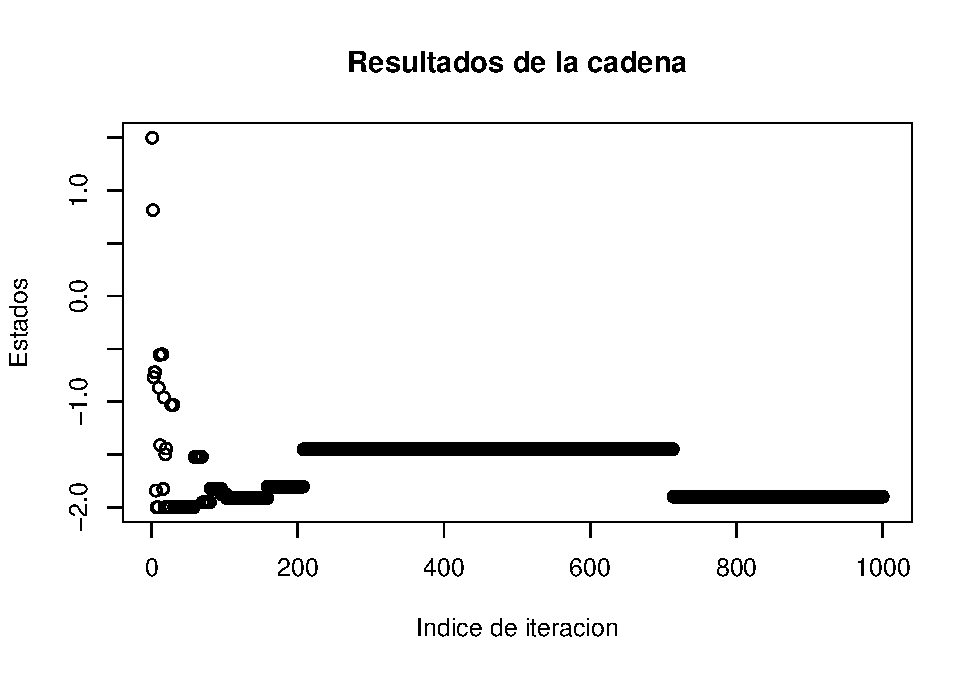
\includegraphics{tarea2_files/figure-latex/unnamed-chunk-14-1.pdf}

\begin{enumerate}
\def\labelenumi{\alph{enumi}.}
\setcounter{enumi}{2}
\item
  Estime la media de la distribución resultante de \(𝑍\).\\
  La media de mcmc es: 1.9555262
\item
  Gráfique el Traceplot de muestra MCMC del algoritmo junto con las
  medias de \(𝑋_1\),\(𝑋_2\),\(𝑍\).
\end{enumerate}

\begin{Shaded}
\begin{Highlighting}[]
\CommentTok{\#Traceplot}
\FunctionTok{plot}\NormalTok{(mcmc,}\AttributeTok{type=}\StringTok{"l"}\NormalTok{,}\AttributeTok{xlab =} \StringTok{"x"}\NormalTok{, }\AttributeTok{ylab =} \StringTok{"y"}\NormalTok{, }\AttributeTok{main =} \StringTok{"Traceplot de muestra MCMC"}\NormalTok{)}
\FunctionTok{abline}\NormalTok{(}\AttributeTok{h=}\NormalTok{mu, }\AttributeTok{col=}\StringTok{\textquotesingle{}blue\textquotesingle{}}\NormalTok{, }\AttributeTok{lwd=}\DecValTok{3}\NormalTok{)      }\CommentTok{\#Media de X1}
\FunctionTok{abline}\NormalTok{(}\AttributeTok{h=}\NormalTok{mu}\SpecialCharTok{/}\DecValTok{2}\NormalTok{, }\AttributeTok{col=}\StringTok{\textquotesingle{}red\textquotesingle{}}\NormalTok{, }\AttributeTok{lwd=}\DecValTok{3}\NormalTok{)     }\CommentTok{\#Media de X2}
\FunctionTok{abline}\NormalTok{(}\AttributeTok{h=}\NormalTok{media, }\AttributeTok{col=}\StringTok{\textquotesingle{}violet\textquotesingle{}}\NormalTok{, }\AttributeTok{lwd=}\DecValTok{3}\NormalTok{) }\CommentTok{\#Media de Z}
\end{Highlighting}
\end{Shaded}

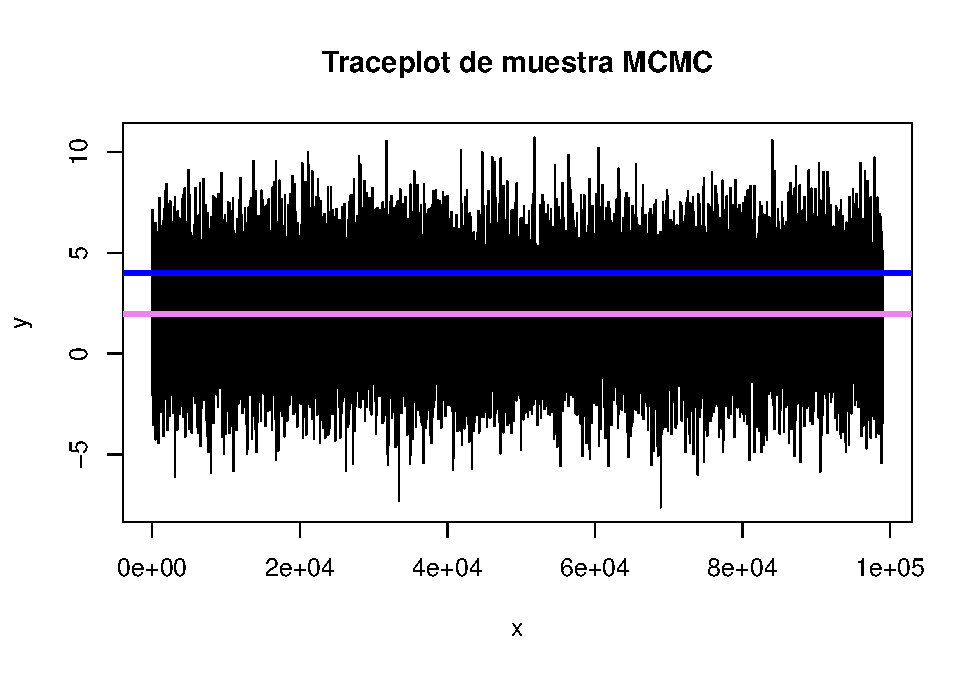
\includegraphics{tarea2_files/figure-latex/unnamed-chunk-15-1.pdf}

\begin{enumerate}
\def\labelenumi{\alph{enumi}.}
\setcounter{enumi}{4}
\tightlist
\item
  El gráfico de Autocorrelación de la muestra MCMC del algoritmo.
\end{enumerate}

\begin{Shaded}
\begin{Highlighting}[]
\CommentTok{\#Grafico de Autocorrelación}
\FunctionTok{acf}\NormalTok{(mcmc,}\AttributeTok{main =} \StringTok{"Autocorrelacion de muestra MCMC"}\NormalTok{)}
\end{Highlighting}
\end{Shaded}

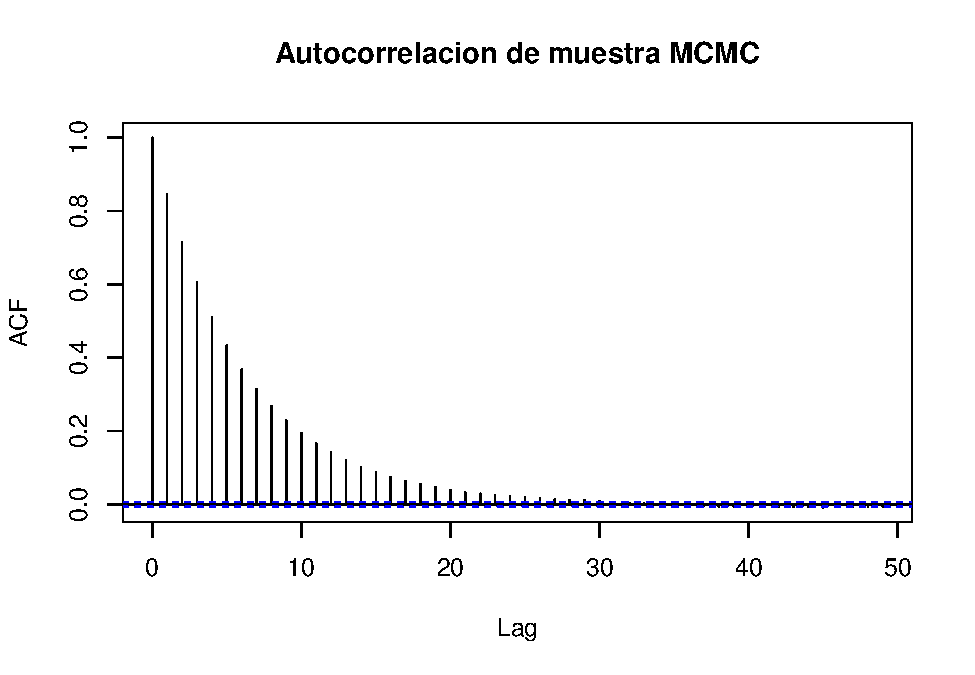
\includegraphics{tarea2_files/figure-latex/unnamed-chunk-16-1.pdf}

\begin{Shaded}
\begin{Highlighting}[]
\FunctionTok{par}\NormalTok{(}\AttributeTok{mfrow=}\FunctionTok{c}\NormalTok{(}\DecValTok{1}\NormalTok{,}\DecValTok{1}\NormalTok{))}
\end{Highlighting}
\end{Shaded}

\begin{enumerate}
\def\labelenumi{\alph{enumi}.}
\setcounter{enumi}{5}
\tightlist
\item
  El gráfico de la convergencia de la media de la muestra MCMC del
  algoritmo.
\end{enumerate}

\begin{Shaded}
\begin{Highlighting}[]
\CommentTok{\#Grafico convergencia de la media}
\NormalTok{m}\OtherTok{=}\NormalTok{N}\SpecialCharTok{{-}}\NormalTok{L}
\NormalTok{acumulado}\OtherTok{\textless{}{-}}\FunctionTok{cumsum}\NormalTok{(mcmc)}\SpecialCharTok{/}\NormalTok{(}\DecValTok{1}\SpecialCharTok{:}\NormalTok{m)}
\FunctionTok{plot}\NormalTok{(}\DecValTok{1}\SpecialCharTok{:}\NormalTok{m,acumulado,}\AttributeTok{col=}\StringTok{"blue"}\NormalTok{,}\AttributeTok{type=}\StringTok{"l"}\NormalTok{,}\AttributeTok{ylab=}\StringTok{"promedio"}\NormalTok{,}\AttributeTok{xlab=}\StringTok{"Iteraciones"}\NormalTok{)}
\end{Highlighting}
\end{Shaded}

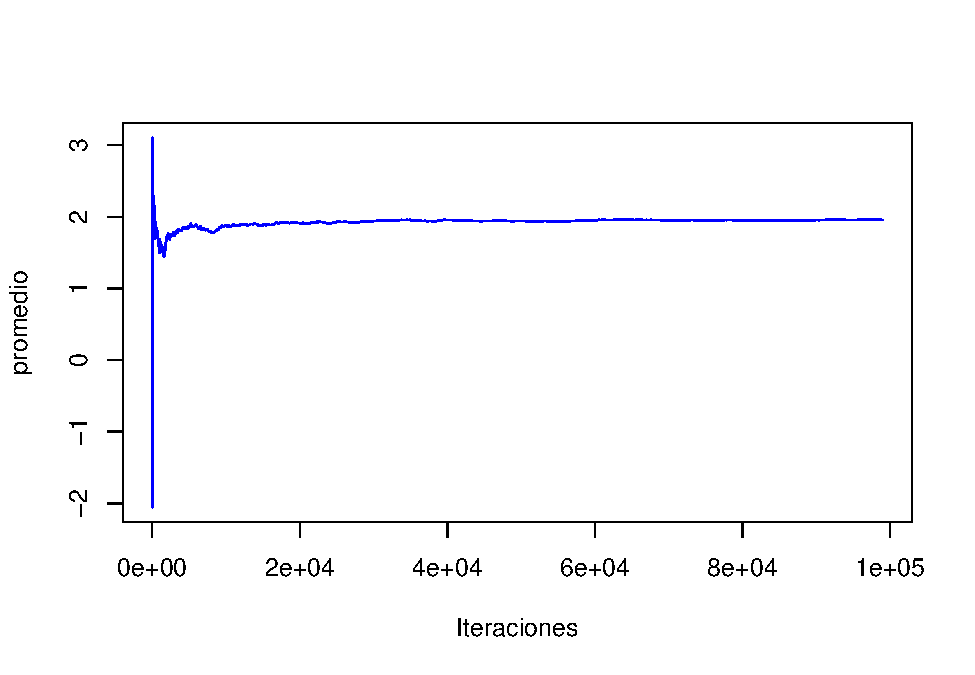
\includegraphics{tarea2_files/figure-latex/unnamed-chunk-17-1.pdf}

\begin{enumerate}
\def\labelenumi{\alph{enumi}.}
\setcounter{enumi}{6}
\tightlist
\item
  La tasa de aceptación del algoritmo.
\end{enumerate}

\begin{Shaded}
\begin{Highlighting}[]
\FunctionTok{cat}\NormalTok{(}\StringTok{"Tasa de aceptación }\SpecialCharTok{\textbackslash{}n}\StringTok{"}\NormalTok{,}
    \StringTok{"NumeroSaltos/TotalIteraciones :"}\NormalTok{ , }\FunctionTok{mean}\NormalTok{(MCMC[,}\StringTok{"Salto"}\NormalTok{]) ,}\StringTok{"}\SpecialCharTok{\textbackslash{}n}\StringTok{"}\NormalTok{)}
\end{Highlighting}
\end{Shaded}

\begin{verbatim}
## Tasa de aceptación 
##  NumeroSaltos/TotalIteraciones : 0.70926
\end{verbatim}

\end{document}
